\documentclass[times, utf8, zavrsni]{fer}
\usepackage{booktabs}
\usepackage{appendix}
\usepackage{algpseudocode}
\usepackage{algorithm}
\usepackage{subcaption}
\usepackage{tocloft}
\usepackage{pdfpages}

\newcommand{\argmax}{\arg\!\max}
\newcommand{\argmin}{\arg\!\min}

\begin{document}

\thesisnumber{3743} 

\title{Information propagation in online social networks}

\author{Iva Miholić}

\maketitle

\includepdf[pages={1,2}]{izvornik.pdf}
\zahvala{
Firstly, I wish to thank my advisor, Asst. Prof. Mile  Šikić for great support and valuable guidance. Thank you to Nino Antulov-Fantulin and Matija Piškorec from Ruđer Bošković Institute in Zagreb for numerous advice and suggestions. Also special thanks to Bruno Rahle for contributing greatly in the data collection.}

\tableofcontents
\clearpage
\listoffigures
\listoftables

\chapter{Introduction}

A \emph{network} is a set of items with connections between them. The Internet, the World Wide Web, social networks like genealogical trees, networks of friends or co-workers, biological networks like epidemiological networks, networks of citations between papers, distribution systems like postal delivery routes: they all take a form of networks. Most social, biological and technological networks have specific structural properties. Such networks are referred to as \emph{complex networks}. Two well-known and much studied classes of complex networks are \emph{scale-free networks} and \emph{small-world networks} whose discovery and definition are canonical case-studies in the field. Both are characterized by specific structural features like power-law degree distributions for the former and short path lengths and high clustering for the latter. An example of a complex network is represented on the Figure \ref{net}.

\begin{figure}[htp]
\centering
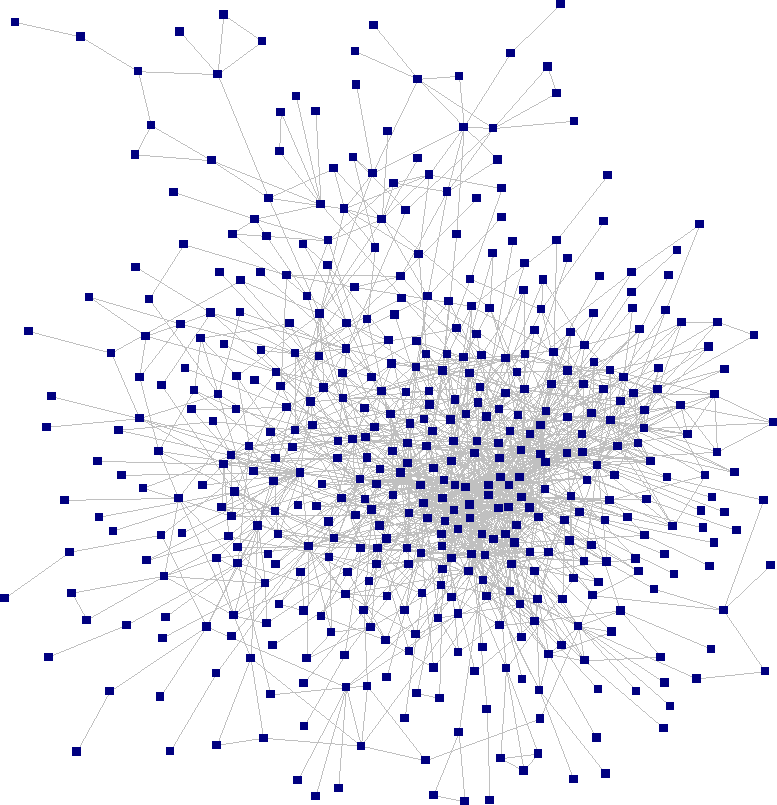
\includegraphics[scale = 0.3]{figs/alters2.png}
\caption{A network graph of Paul Erd\~os and his collaborators, courtesy of \cite{krebs}. The nodes represent mathematicians and the edges represent the relationship "wrote a paper with".}
\label{net}
\end{figure}
A network structure or a topology can be mathematically modeled as a graph with set of vertices (or nodes) representing the items of the network. The network structure can then be analyzed using graph theory. An edge between two nodes represents a connection between the two corresponding items. Edges can be directed or undirected, weighted or unweighted, depending  on the nature of the connection.  To better mimic the real-world (complex) network structure, it is common to add attributes to nodes and/or edges or to have both directed and undirected edges on the same graph.

For large-scaled complex networks that have millions or billions of vertices, the study in the form of traditional graph theory is not sufficient or sometimes possible. When this is the case, the statistical methods  for quantifying large complex networks are used. 

The ultimate goal of the study of complex network structure is to understand and explain the processes that take place on the network topology such as spreading of diseases or information propagation in social networks.

After statistical properties analysis, the model of a complex network is created. The model can help us understand the meaning of statistical properties - how they came to be as they are and how they relate to the behaviour of a networked system. Based on the statistical properties and using the right model, the behavior of networked systems can be predicted.

The basis of the complex network theory; the structure  analysis and the process modeling can be found in \cite{Newman03thestructure}.

\chapter{Online social networks and information propagation}

A complex network of profile pages and connections between them created by      users of social networking sites such as Facebook and Twitter is refered to as \emph{online social network}. Through these networks, users can communicate and share information. Since online social networks allow hundreds of millions of Internet users worldwide to produce and consume content, the structure of these social networks represents a huge amount of data that can be used  to extract important information about the systems built upon the network. 

An online social network's structure is also formally represented by a graph where nodes are users and edges are relationships between them. Direction of edges depends on the social networking site's social model. For example, Facebook's social model of \emph{friendship} connects in bilateral and Twitter's model of \emph{following} connects in unilateral manner. 

When there is an edge between two nodes, users corresponding to that nodes may exchange messages. One user can send messages to all of its connections at once or he can send a message to one user at once, depending on the social networking site's social model. Users publish messages to share or forward various kind of information.

\section{Information propagation}

\emph{Information item} is a news item or an idea that propagates amongst nodes contained in the body of messages. We refer to the nodes that have adopted a  particular item as \emph{active} and the nodes that have not adopted the same item as \emph{inactive}. The activated nodes never deactivate. It is important to define when exactly the node became active, \emph{i.e.} has adopted the information item.


 When talking about information adoption for a particular node, some authors \cite{leskovec} distinguish between \emph{exposure event} and \emph{infection event}. \emph{Exposure event} occurs when a node gets exposed to the information item, in other words, when the user reads a received message containing the information item. On the other hand, \emph{infection event} occurs when a message is sent. Every exposure may lead to infection event. 
 
With the given network structure and a stream of messages with corresponding content, timestamp, sender and receivers that are sent on the network, the times of all infection events are known. In other words, from such data we can only know exposure has happened sometime before the recorded infection event. Exposures that  didn't lead to infection remain unknown. Additionally, one node can be exposed multiple times before the recorded infection. The frequency of those exposures is unknown. For simplicity, we will consider a node as active when it gets infected.

\section{Social influence and information diffusion}

The term \emph{diffusion} in natural sciences refers to the net movement of a substance from a region of high concentration to a region of low concentration. When a message containing some information item is sent, receivers may or may not choose to send a message containing the item to their other connections. 

The action of adopting and resharing some particular information item is a decision based on the action of the previous message sender, therefore, individuals are influenced by the actions taken by others. This social phenomenon when actions of a user can induce his connections to behave in a similar way is known as \emph{social influence}. 

The stream of messages that carries the same information item among the nodes of the social network driven by  \emph{social influence} causes the information to be adopted in a similar way as the molecules of dye diffuse  in water. The described spread of information caused by social influence is therefore known as \emph{information diffusion}.

\section{External influence}

When a user adopts particular information item, it is important to ask where did the information item  initially came from. If we assume a closed-world model with initially active set of nodes, we can categorize all information adoptions  as social influence driven. However, the online social network is not a closed world and exposure to an information item can originate from some other sources. 

Due to emergence of mass media, especially online news sites, the information can reach nodes of online social network driven by the influence of exogenous out-of-network sources, as well as by the social influence. Depending on the strength of exogenous influence, the process of adopting information on the social network no longer resembles diffusion. 

With greater external influence, more and more users whose connections didn't yet adopt the observed information become exposed  and infected. This particular kind of adoption can only be explained by the influence of some unobserved exogenous source. However, if it is known the exogenous source exists and the node has neighbours that have already adopted the observed information item, we are not sure whether the adoption of information for that node is due to exogenous or social influence.

The focus of this thesis is to present a model of information propagation with both internal (social) and external influence developed in \cite{authority} and use it to classify whether the adoption of a particular item of information for the given network is mainly internal or external influence driven.

\chapter{Referendum Dataset}

  On $1^{st}$ of December 2013 referendum on the question "Do you support constitutional amendment about marriage  being community of man and woman" was held in Croatia. A week before, starting from 25th of November, Facebook application referendum2013.hr \cite{ref} became active. Once the user registered, he/she could answer the same referendum question and see how his/hers Facebook friends have answered.
  
  With users consent, using the application the demographics data, timestamps of registration and vote casting and the votes of $12763$  registered users were collected, as well as the network of their Facebook friends. The complete network structure of both registered users and their friends contains roughly $1.695$ million nodes with $4.461$ million edges.  
  
The degree distribution for the complete network of registered users only fits the function $x^{-\alpha}$ known as the power-law curve which is a common structural property of complex networks \cite{Newman03thestructure}. The distribution of degrees is shown on the Figure \ref{degs}.

\begin{figure}[htp]
\centering
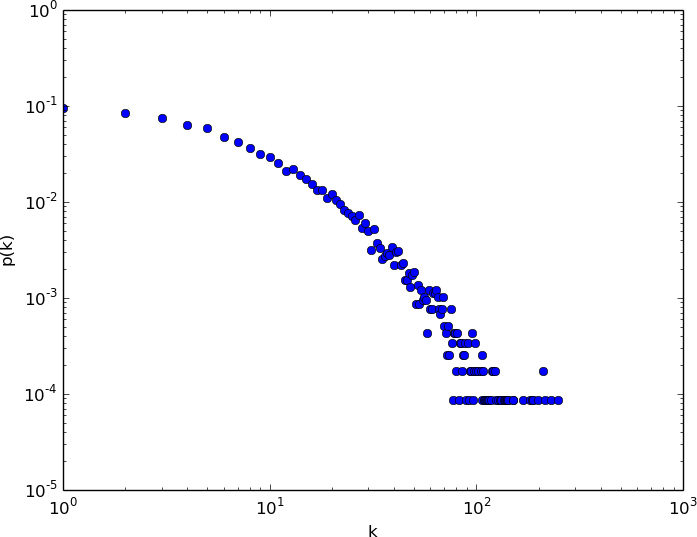
\includegraphics[scale=0.6]{figs/log_mali.png}	
\caption{The degree distribution for the network of registered users. $p(k)$ is the probability that a vertex chosen uniformly at random has degree $k$.}
\label{degs}
\end{figure}

 The majority of users ($72.6$ \%)  who have casted their vote ($11606$ registered users) voted against the support to the definition of marriage as stated in the referendum question. Since that result differs greatly from the official referendum result where $33.5$ \% of $1.446$ million voters voted 'against' the definition of marriage as stated in the referendum question, motivation for performing data analysis and developing models for information propagation arose. 
 
 In this case, information propagation refers to  information on the existence of the application that  spread among the network of users via link sharing through Facebook's social model of \emph{sharing} or directly. The timestamps of registrations indicate the times of adoption of that information item but how the adoption has happened remains unknown.  
   
 Along with the network of users and their Facebook friends, major online media coverage was observed and documented in the form of articles  along with its timestamps of publishing.
 
 The majority of peaks in voting activity dynamics align with the $11$ documented article timestamps, but the role of media in engaging the voters has to be confirmed with a model. 
 
For simplicity, we will assume every media article had the same chance of influencing every recorded user and the users did not influence the media. With this assumptions, the network of media nodes is completely influentially separated from the user nodes, while the user nodes are not influentially separated from the media. Since that is the case, it is reasonable to think of media nodes as a complete graph of nodes that somehow exchange information between themselves.    
 
\section{Datasets}
\emph{Referendum Dataset} represents two network structures we will refer    to as  \emph{Restricted} and \emph{Complete Referendum Dataset}. 
The \emph{Restricted Referendum Dataset} consists of two subgraphs. The first subgraph has $12763$ nodes representing the registered users. If two users are Facebook friends, there exists a bilateral connection between the two corresponding nodes. Every node also carries the  registration timestamp as a node attribute. 

The nodes of the second subgraph correspond to $11$ recorded mass media articles. These nodes also carry the information about the timestamp of activation as a node attribute (the node is activated when the article got published). Every node in second subgraph has a bilateral edge with every other node in the subgraph. The two subgraphs are connected unilaterally: every node  representing the media (from the  second subgraph) has edges directed to every node representing a user (but not vice versa).

By extending the first subgraph with nodes representing the Facebook friends of registered users that did not  register, network structure we will refer to as \emph{Complete  Referendum Dataset} is obtained. 

The Complete Referendum Dataset consists of $1695421$ nodes representing the users and their friends with $4461556$ bilateral edges connecting them. The second subgraph that represents the media is exactly the same as in the \emph{Restricted Referendum Dataset}. Additionally, the set of  unilateral edges connecting  the nodes of the second subgraph to the nodes of the first subgraph is extended by the set of unilateral edges connecting every node representing the media to every node in the first subgraph that represents an unregistered friend of registered user(s).

The anonymized network of user nodes with corresponding timestamps of activation is stored in GML format \cite{gml} while the media nodes and other mentioned connections are defined implicitly.
  
\chapter{Methods}
\section{Principle of maximal likelihood}

A \emph{statistical model} $S_X(\theta)$ is a family of parametrized probability distributions defined for a set of real-valued parameters represented by vector $\theta$ and continuous or discrete random variable $X$. The distribution can be described  as a probability mass function $F_X(x;\theta) = P(X = x)$ or a probability density function $f_X(x;\theta) = \frac{d}{dx}F_X(x;\theta)$. With given training set and a statistical model, the principle of maximal likelihood is used to reduce the problem of choosing the distribution from $S_X(\theta)$ for the given training set, what is known as \emph{model fitting}, to the maximization or a minimization problem.

 \emph{Random sample} is a set of $m$ observations, examples or outcomes $x_1, x_2,$ $\dots, x_m$ drawn from the fixed but unknown distribution in $S_X(\theta)$. Suppose that we have a random sample drawn. If we assume the examples are independant, the probability of a random sample is the product of probabilities for the individual examples with some fixed parameters $\theta$:

\begin{equation}
\label{fxt}
 f(x_1, x_2, \dots, x_m; \theta) = \prod_{j=1}^{m}{f_{X}(x_j; \theta )}. 
\end{equation}

The function $L(\theta; x_1, x_2, \dots, x_m) = f(x_1, x_2, \dots, x_m; \theta)$ defined like \eqref{fxt} but considered as the function of $\theta$ depending on $m$ fixed parameters $x_1, x_2, \dots, x_m$ is a \emph{likelihood function}. It is used to compare how different members of the statistical model fit the training data. 

\emph{The principle of maximal likelihood} says that for the given random sample (training data or a dataset), we should use as a model the distribution from $S_X(\theta)$ that gives the greatest possible probability to the training data. Since the vector $\hat\theta$ that maximizes the probability of the traning data also maximizes the likelihood function $L$, it is obtained using the following equation:
\begin{equation}
\label{MLE}
 \hat\theta = \argmax_{\theta} L(\theta; x_1, x_2, \dots, x_m).
\end{equation}

The vector $\hat\theta$ is refered to as \emph{the maximum likelihood estimator (MLE)} of parameters $\theta$. 

\emph{The log likelihood function} $l(\theta; x_1, x_2, \dots, x_m)$ is the logarithm of the likelihood function $L(\theta)$. Since logarithm is a monotonic strictly increasing function, maximizing the log likelihood over all possible values of vector $\theta$ is equivalent to the maximization problem stated in \eqref{MLE}. Additionally, minimization of negative log likelihood is also equivalent to \eqref{MLE}.

When we want to determine $\hat\theta$ for the given dataset, we will choose between solving the problem of maximizing the likelihood, maximizing log likelihood or minimizing negative log likelihood.

\subsection{Conditional likelihood}

For two discrete random variables $X$ and $Y$, conditional probability is formally defined as 
\begin{equation}
\label{cond}
	p(y | x) = P(Y = y | X = x) = \frac{P(Y = y, X = x)}{P(X = x)}. 
\end{equation}
We can say that \eqref{cond} denotes the probability of a value $y \in Y$ when the value of $X$ is known. If the variables are dependant, $Y$ follows a probability distribution that is different for different values of $X$. We parametrize all these probability functions with the same vector of parameters $\theta$.

The conditional likelihood of $\theta$ given data $x \in X$ and $y \in Y$ is 
\begin{equation}
	L(\theta;y | x) = P(Y = y | X = x; \theta ).
\end{equation}

For finding the conditional likelihood estimator, the random sample consists of $m$  pairs $\{(x^{(i)}, y^{(i)}) | 1 \le i \le m\}$. If  all $y^{(i)}$ are independent when each is conditioned on its own $x^{(i)}$, we can define probability of the random sample as a product of probabilities for all pairs $\{(x^{(i)}, y^{(i)}) | 1 \le i \le m\}$ from the random sample, similar to \eqref{fxt}:
\begin{equation}
\label{fxt2}
 L(\theta; y_1|x_1, y_2 | x_2, \dots y_m | x_m) = \prod_{i=1}^{m}{P(Y = y_i | X = x_i;\theta)}    . 
\end{equation}

After determining $\hat\theta$, we can use it to compute probabilities for the alternative values $y \in Y$ given any specific value of $x$. The procedure with this feature is called a \emph{classifier}.

\section{Gradient descent algorithm}

The gradient descent algorithm can be used as an iterative optimization method for solving minimization problems that cannot be solved directly.

Let's say we want to find the values of parameter vector $\theta$ of $n$  parameters, $\hat \theta \in \mathbf{R}^n$, that minimizes function $f(\theta)$. Given the \emph{gradient vector} of $n$ partial derivates $\frac{\partial}{\partial \theta_j} f(\theta)$  with respect to each parameter $\theta_j$, $1 \le j \le n$ from $\theta$, the \emph{gradient descent} starts  from random $\theta$, and at each step simultaneously updates the values $\theta_j$ for all $1 \le j \le n$ in the opposite direction of the gradient:
\begin{equation}
\theta_j = \theta_j - \alpha \frac{\partial}{\partial \theta_j} f(\theta).
\end{equation}

The coefficient $\alpha$ refers to the \emph{stepsize} or a \emph{learning factor}. It  determines how much to move in the direction given by the negative value of the derivative.

When the procedure finds the vector $\theta$ that minimizes $f(\theta)$, partial derivatives will evaluate to $0$ and the procedure will terminate. Thus, procedure will find the local minimum but there is no guarantee of finding the global minimum if the function $f(\theta)$ is not unimodal. The use for the good value of $\alpha$ is also critical: the algorithm will converge slowly with small $\alpha$ and  a large value of $\alpha$ may cause the algorithm not to find the nearest local optimum or it may even cause divergence. 

Pseudocode for the described algorithm is given below as Algorithm \ref{algo1}.  
\begin{algorithm} 
\caption{The Gradient Descent Algorithm}
\label{algo1}
\begin{algorithmic}
\For{$j=0$ to $n$}    
    \State $\theta_j \gets rand(0, 1)$
\EndFor
\Repeat
\State $\theta' \gets \theta$
\For{$j=1$ to $n$}
\State $\hat \theta'_j \gets \hat \theta'_j - \frac{\partial}{\partial \theta_j}f(\theta)$  
\EndFor
\State $\theta  \gets \theta'$    
\Until{convergence} \\
\Return $\; \theta$
\end{algorithmic}
\end{algorithm}

It is best to initialize $\theta$ with random values  close to $0$. If the initial values of $\theta$ are large in magnitude, the procedure may also not find the nearest local optimum.
    
\subsection{BFGS}
\emph{Broyden-Fletcher-Goldfarb-Shanno algorithm} (BFGS) is an example of advanced iterative method for solving unconstrained nonlinear optimization problems. 

Similarly to the gradient descent algorithm, this method uses both first and second order  derivatives of the function for the update. Since BFGS has been proven to have good performance even for non-smooth optimizations, it will be used for optimizations in this paper. 

During the optimization, the first order derivative has to be evaluated directly, unlike second order derivatives in the form of Hessian matrix. The Hessian matrix can be approximated using the gradient evaluations. BFGS also finds acceptable stepsize $\alpha$  for every iteration.

\section{Logistic regression}
Suppose $Y$ is a binary (Bernoulli) outcome and that $x \in X$ is a  real-valued vector with $n$ values $x_1, x_2, \dots, x_n$. We model the probability that $Y = 1$ as a nonlinear function of a linear function of $x \in \mathbf{R}^n$ with unknown real-valued vector of parameters $\theta \in \mathbf{R}^{n + 1}$ using logistic regression.

\emph{Logistic regression} is a model with conditional probability functions defined as:
\begin{equation}
\label{reg}
	P(Y = 1 | X = x; \theta) = \sigma(\theta_0 + \sum_{j = 1}^{n} \theta_j  x_j) = \frac{1}{1 + \exp(-\theta_0 - \sum_{j = 1}^{n} \theta_j  x_j)}
\end{equation}
with $x \in \mathbf{R}^n$ and $\theta \in \mathbf{R}^{n + 1}$.

The function $\sigma(z) = \frac{1}{1 + e ^ {-z}}$ is nonlinear always-increasing function  and it is commonly known as \emph{the sigmoid function}. The graph of the sigmoid function is shown in the Figure \ref{sig}.
\begin{figure}[htp]
\centering
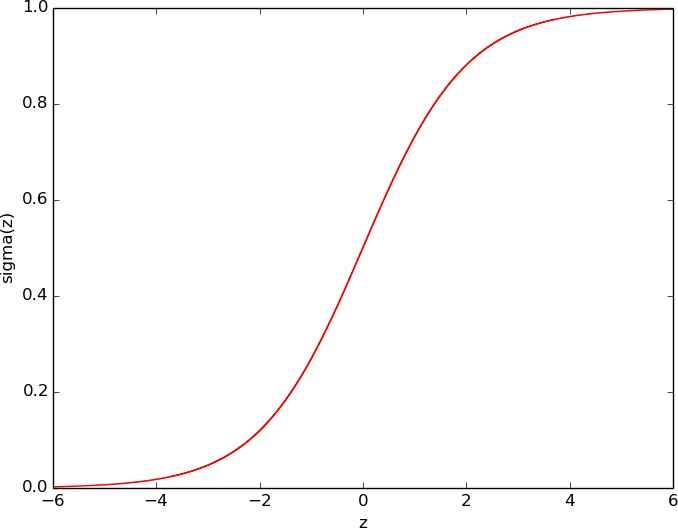
\includegraphics[scale=0.59]{figs/sig.png}
\caption{Function $\sigma(z) = \frac{1}{1 + e ^ {-z}}$.}
\label{sig}
\end{figure}

The logistic  regression model is easier to understand in the form of the log odd:
\begin{equation}
\log \frac{p}{1 - p} = \theta_0 + \sum_{j = 1}^n \theta_j x_j
\label{logodds}
\end{equation}
where $p$ is an abbreviation for $P(Y = 1 | X =x; \theta)$.

The odds of event Y = 1 given  X = x is exactly the ratio $\frac{p}{1 - p}$.  Since probabilities range from $0$ to $1$, odds range from $0$ to $\infty$ and log odds, $\log\frac{p}{1 - p}$, range from $-\infty$ to $\infty$. A linear expression on the right hand side of \eqref{logodds} can also take unbounded values so it is reasonable to use  a linear  expression as a model for log odds.

Logistic regression is the simplest reasonable model for a random binary outcome whose probability depends linearly on $n$ features represented by the feature vector $x \in \mathbf{R}^n$.  The limitation of the basic logistic regression model is that the probability must either increase monotonically or decrease monotonically as a function of each feature $x_j \in x, 1 \leq j \leq n$. To extend the model for polynomial dependencies, feature vector can be extended with higher-order polynomial factors of the original features. 

\subsection{Logistic regression classifier}
For the given vector of features $x \in \mathbf{R}^n$ drawn from the distribution of a multidimensional random variable $X$, we want to predict a binary response from the binary predictor $Y$ dependent on $X$. The dependency (the conditional probability) is modeled as a logistic regression. To learn a logistic regression classifier we must choose parameter values $\hat\theta$ that best fit the training set data. Once training is complete and $\hat\theta$ is obtained, we use thus defined conditional probability to make further predictions: the value of $Y$ is predicted as $1$ if the probability of $P(Y = 1| X = x) \geq 0.5$ for the input feature vector $x$, otherwise it is predicted as $0$.

Given the training set of $m$ training example pairs $\{(x^{(i)}, y^{(i)}) \; | \; 1 \le i \le m\}$, the logistic regression classifier is learned by  minimizing the negative conditional log likelihood.
 
Taking the logarithm of \eqref{fxt2} and negating gives the expression for the negative conditional log likelihood, $NCL(\theta)$:
\begin{equation}
NCL(\theta) = \sum_{i = 1}^{m} -\log L(\theta;y_i|x_i) = \sum_{i = 1}^{m} -\log p(y_i | x_i; \theta)
\label{NCL}
\end{equation}

If we denote $P(Y = 1 | X = x_i; \theta)$ as $p_i$, the probability of the training example pair $(x^{(i)}, 1)$ is exactly $p_i$, while the probability of the example $(x^{(i)}, 0)$ is $1 - p_i$.  Now we can simplify the above equation as \begin{equation}
NCL(\theta)  = \sum_{i;y=1} -\log p_i + \sum_{i;y=0} -\log (1 - p_i)
\end{equation}

The  problem of minimizing $NCL(\theta)$ can now be defined similarly to \ref{MLE}:
\begin{equation}
\label{LMLE}
 \hat\theta = \argmin_\theta (-{\sum_{i;y = 1} \log p_i - \sum_{i;y=0} \log(1 - p_i)})
\end{equation}

Because of the nonlinearity of the sigmoid function, the minimization problem stated in \eqref{LMLE} cannot be solved directly, therefore optimization techniques are used. 

Derivatives of the $NCL(\theta)$ with respect to every parameter in $\theta$ have to be determened in order to use previously described optimization techniques.

The partial derivative of $NCL$ \eqref{NCL}  with respect to parameter $\theta_j$ is    
\begin{equation*}
\frac{\partial}{\partial \theta_j} NCL(\theta) = -\sum_{i;y = 1} \frac{1}{p_i} \frac{\partial}{\partial \theta_j} p_i - \sum_{i;y = 0} \frac{1}{1 - p_i} (-\frac{\partial}{\partial \theta_j} p_i)
\end{equation*}

With $p_i = \frac{1}{1 + e^{-z}}$ where $z = \theta_0 + \sum_{j=1}^{n} \theta_j$, we have
\begin{equation}
\frac{\partial}{\partial \theta_j} p_i = \frac{e^{-z}}{(1 + e^{-z})^2} \frac{\partial}{\partial \theta_j} z = p_i (1 - p_i) x_j \
\label{logp1}
\end{equation}
for $0 \le j \leq n$ and for $j = 0$,
\begin{equation*}
\frac{\partial}{\partial \theta_0} p_i = p_i (1 - p_i).
\label{logp2}
\end{equation*}

Hence, $\frac{\partial}{\partial \theta_j} \log p_i = (1 - p_i) x_j$ and $\frac{\partial}{\partial \theta_j} \log (1 - p_i) = - p_i x_j$ with additional extension of vector $x$ with $x_0 = 1$.

The derivation for the entire dataset is easily derived as the sum of the corresponding partial derivatives of the examples:  
\begin{equation}
    \frac{\partial}{\partial \theta_j} NCL = -\sum_{i;y = 1} (1 - p_i)x^{(i)}_j - \sum_{i;y = 0} -p_i x^{(i)}_j = -\sum_{i}(y_i - p_i)x^{(i)}_j
\end{equation}

Notation $x^{(i)}_j$ refers to the $j$-th feature of the $i$-th feature vector $x^{(i)}$ in the random sample.


\chapter{Modeling information propagation with internal and external influence}
\section{Modeling the structure of the network}

Formally, information propagation network can be represented as a graph $G=(V,E)$. We refer to elements of set $V$ as vertices, nodes or \emph{peers}. Every edge $(u, v) \in E$ from node $u$ to node $v$ denotes that node $u$ can (socially) influence node $v$. In other words, every neighbour of node $u$ can be influenced by $u$. We call graph $G$ the \emph{peer influence graph}. 

We extend graph $G$ with a set $A$ of \emph{external nodes} or \emph{authorities}. Every authority $a \in A$ can potentially influence every node in $V$ but not vice versa.  That is, every authority $a \in A$ is connected to every node $v \in V$ and can influence it. This influence is not social and it was previously  referenced to as external influence. Additionally, the subgraph $A$ is fully connected, \emph{i.e.} every node $a \in A$ is connected bilaterally with all nodes $b \in A$ if $a \neq b$. If we use $F$ to represent the directed edges from authorities to peers, we can define new a graph $H = (V \cup A, E \cup F)$,  the \emph{extended influence graph}. 

\section{Modeling the process of information propagation}
 
 Information item propagates between both peer and external nodes. If a particular node (peer or authority) has adopted an item, we refer to it as \emph{active}. We call the nodes that  have not adopted the same item as \emph{inactive}. 
 
The actual propagation process can be observed as successive activation of nodes throughout the network that we refer to as the  \emph{activation sequence}. Structure representing the activation sequence will be a set of nodes along with their activation timestamp. To describe the propagation process, we construct a new set of nodes $D$. A node $u \in V \cup A$ is in $D$ if its activation time  is recorded. Every node in $D$ has an attribute $t$ --- the activation timestamp.    

We assume the propagation of a particular information item happens in discrete time steps, from timestamp $1$ to timestamp $T$. At every point in time, $t \in \{1, 2, \dots, T\}$, each inactive node can become active with probability $P(x, y)$. This probability is a function of $x$ --- the number of neighbours  of the observed node that became active before time $t$ and $y$ --- the number of external nodes that became active before time $t$.

For every timestamp $t \in \{1, 2, \dots, T\}$ and every currently inactive node $u$, an event of $u$ adopting the information is observed. The success of this event is a  Bernoulli random variable. If an event is successful, the node becomes active at that time. All successful events are listed in the activation sequence. We will use the logistic regression to model the probability $P$ and determine the parameters of this distribution based on the activation sequence and the network $H$. That is, the probability $P$ is defined as:

\begin{equation}
\label{Pxy}
 P(x, y; \alpha, \beta, \gamma) = \frac{1}{1 + e ^ {-\alpha \ln(x + 1) - \beta \ln(y + 1) - \gamma}},	
\end{equation}

where $\alpha$, $\beta$ and $\gamma$ are the parameters of logistic regression. The parameter $\gamma$ takes the role of $\theta_0$ in \eqref{reg}.

The arguments (features) $x$ and $y$ come into linear transformation in the argument of the sigmoid function transformed with the $\ln$ function.  That will help in further analysis of retrieved  values of $\alpha$ and $\beta$ since $\ln(x+1)$ and $\ln(y + 1)$ have a similar range of values.  

The value of $\alpha$ in \eqref{Pxy} captures the strength of social influence in the propagation of an information item, while the value of $\beta$ captures the strength of external (authority) pressure. We refer to $\alpha$ and $\beta$ as \emph{peer coefficient} and \emph{authority coefficient}, respectively. Parameter $\gamma$ models the impact of other factors in the propagation of an information item, such as daytime dynamic, effect of random chance and other noises. We call $\gamma$ the \emph{externality coefficient}. 

\subsection{Information propagation model training}
We estimate $\alpha$, $\beta$, and $\gamma$ by learning the logistic regression classifier using negative log likelihood function. 

To calculate the likelihood, we first define the number of nodes that at the beginning of time $t$ had $x$ active influencing neighbors and they themselves became active at time $t$ when $y$ authorities were active as $A(x, y, t)$. Similarly, let $N(x, y, t)$ be the number of users who at the beginning of time $t$ had $x$ active influencing neighbors and they did not became active at time $t$ when $y$ authorities were active. Let $A(x, y) = \sum_{t = 1}^{T}A(x, y, t)$ and $N(x, y) = \sum_{t=1}^{T}N(x, y, t)$. 

The maximum-likelihood estimation of parameters $\alpha$, $\beta$ and $\gamma$ are those that maximize the likelihood of the data at time $t$. If every inactive node $u$ is  characterized by two metrics, $x$ and $y$,  $\; L(\alpha, \beta, \gamma)$ is defined as
\begin{equation}
\label{LF}
 L(\alpha, \beta, \gamma) = \prod_{x, y} P(x, y) ^ {A(x, y)} (1 - P(x, y)) ^ { N(x, y)}.
\end{equation}

In the next step, the problem of finding the arguments $\alpha, \beta, \gamma$ that maximize \eqref{LF} is reduced to minimization of negative log likelihood, just like in the general steps of learning the logistic regression classifier:

\begin{equation}
\centering
\begin{split}
 -\ln L(\alpha, \beta, \gamma) = -\sum_{x, y} \ln P(x, y) ^ {A(x, y)} - \sum_{x, y} \ln(1 - P(x, y)) ^ {N(x, y)}   \\ = -\sum_{x, y} A(x, y) \ln P(x, y) - \sum_{x, y} N(x, y) \ln (1 - P(x, y)). 
\end{split}
\end{equation}

The derivatives with respect to $\alpha$, $\beta$ and $\gamma$ of the same function were derived from \eqref{logp1} and \eqref{logp2} and are as follows: 
\begin{equation}
\frac{\partial}{\partial \alpha}(-\ln L)= 
 \sum_{x, y}  \left[ -A(x, y) (1 - P(x, y)) + N(x, y) P(x, y) \right] \ln(x + 1),
\label{dera}
\end{equation}
\begin{equation}
\frac{\partial}{\partial \beta }(-\ln L) = \sum_{x, y} \left[ -A(x, y)  (1 - P(x, y)) + N(x, y)P(x, y) \right] \ln(y  + 1),
\label{derb}
\end{equation}
\begin{equation}
\frac{\partial}{\partial \gamma } (-\ln L) = \sum_{x, y} \left[ -A(x, y)  (1 - P(x, y)) +  N(x, y) P(x, y) \right].
\label{derg}
\end{equation}

The only problem remaining is the calculation of $A(x, y)$ and $N(x, y)$ that has to be efficient for a network with million nodes (number of nodes in the Complete Referendum Dataset).

\subsection{Computing $A(x, y)$ and $N(x, y)$}

For the given extended influence graph $H = (V \cup A, E \cup F)$ and the set of activated nodes  $D$, $\; A(x, y)$ and $N(x, y)$ are computed using the following dynamic data structure: There are $M + 1$ buckets where $M$ refers to the maximum number of active neighbours one node could have. The $x^{th}$ bucket   (with notation $bucket[x]$) will during the procedure contain all nodes that at the time had $x$ active neighbours. At the beginning, all nodes are in the $bucket[0]$.
 
Every iteration of the algorithm tracks the dynamic of one time step. Values of $N(x,y)$ and $A(x,y)$ are updated for the current $y$ and all currently possible values of $x$ at every iteration. To correctly count the number of neighbours that became active exactly before time $t$ for every node  that didn't activate before time $t$, two passes through the corresponding nodes in D are needed.

Before the first pass, values of $N$ are updated. Value of $N(x,y)$ is incremented for every node that currently has $x$ active neighbours. Since the $bucket[x]$ stores all nodes with $x$ active neighbours at that time, $N(x,y)$ is incremented by the size of this bucket. This step is correct since the following invariants hold:
\begin{itemize}
\item{at every iteration, one node  is stored in at most one bucket and }
\item{the activated nodes are not in any bucket.}
\end{itemize} 

With this update, the nodes that will become active at currently observed time $t$ are also counted in the values of $N$. This will be corrected in the first pass through the nodes in $D$. When the value of $A(x,y)$ updates for every activating node, corresponding value of $N(x,y)$ decrements. 

In the second pass of nodes in $D$, the data structure of buckets is updated for recently activated nodes and their neighbours. That is, every activated node is removed from the structure and its neighbours are moved to the bucket that corresponds to  one activated neighbour more than they previously had.

Lastly, for every iteration, \emph{i.e.} time step, value of $y$ is updated according to the activation timestamps of the external nodes.

The pseudocode of the described algorithm is given as Algorithm \ref{algo2}. This algorithm assumes the existence of the function $getBucket(node\: u)$ that returns the index of the bucket where node $u$ is currently stored in $\mathcal{O}(\log(|V))$ time.

Assuming all other functions take $\mathcal{O}(1)$ to complete, the time complexity of the algorithm is derived as follows:
\begin{equation*}
\begin{aligned}
\mathcal{O}(|V| \;\;\;\;\;\;\;\;\;\;\;\;\;\;\;\;\; \text{from line}\; 2 \\
          \;    + \;T M  \;\;\;\;\;\;\;\;\;\; \text{from lines} \;4-6 \\
          \;    + \;T \frac{|D|}{T}\ln(|V|)  \;\;\;\;\;\;\;\; \text{from lines} \;7-11 \\
          \;    + \;T \frac{|D|}{T}\left[\ln(|V|) + M\ln(|V|)\right]  \;\;\;\;\;\; \text{from lines} \;12-22 \\
          \;    + \;T |A|) \;\;\;\;\;\; \text{from lines} \; 23-27 \\
\Rightarrow           \mathcal{O}(|V| + M|D|\ln(|V|) + MT + |A|).
\end{aligned}
 \phantom{\hspace{4cm}} 
\end{equation*}

\begin{algorithm}[htp]
\caption{Computing $A(x,y)$ and $N(x,y)$}
\label{algo2}
\begin{algorithmic}[5]
\State $y \gets 0$
\State $bucket[0] \gets V$

\For{$t = 0$ to $T$}
   \For{$x = 0$ to $M$}
       \State $N(x, y) \gets N(x, y) + size(bucket[x])$
   \EndFor
   \For{$u \in D, u.t = t$}
   \State $x \gets getBucket(u)$
   \State $N(x, y) \gets N(x, y) - 1$
   \State $A(x, y) \gets A(x, y) + 1$ 
   \EndFor
   \For{$u \in D, u.t = t$}
   \State $x \gets getBucket(u)$ 
   \State $bucket[x].remove(u)$   
   \For{ $n \in u.neighbours()$}
    \If {$notActive(n)$}     
        \State $x' \gets getBucket(n)$
     \State $bucket[x'].remove(n)$    
     \State $bucket[x' + 1].add(n)$
\EndIf     
     \EndFor
     \EndFor
    \For{$a \in A$}    
    \If{ $a.t = t$ }   
    \State $y \gets y + 1$
    \EndIf 
    \EndFor        
\EndFor \\
\Return $A, N$
\end{algorithmic}
\end{algorithm}

\section{Assumptions of the presented model}
The presented model assumes that the probability of activation for a node grows monotonically with number of activated neighbours as well as with number of active authorities. If the correlation between $x$ and probability of activation were to be negative, the coefficient $\alpha$ would be estimated to some negative value. Similarly, if the correlation between $y$ and probability of activation were to be negative, the coefficient $\beta$ would be estimated to a negative value.

It is reasonable to assume that social influence of an active  node fades away after certain time. That is also true for the external influence in the form of articles at online news sites since the articles aren't always as  accessible as at the time of the publishment. This model assumes the influence of an active node does not fade away with time, \emph{i.e.} the influence of a node, peer or authority, is constant after the activation.

Additionally, this model assumes the time progress in discrete time steps.


\section{Randomization Test}

We choose to infer whether information propagation of an item is better explained due to peer or external influence by obtaining the maximum-likelihood estimates of peer and authority coefficients $\alpha$ and $\beta$. 

It is reasonable to say: if $\alpha > \beta$ than information is peer-propagated, otherwise, if $\alpha <  \beta$, the information item is authority propagated. The question remains, how much larger should the value of $\alpha$ (or $\beta$) be in order to characterize information item as peer- (or authority- ) propagated and how to verify that this result is due to strong evidence in the data.

In order to verify that this kind of conclusion is based on strong evidence in the data, \cite{akm-icsn-kdd08} and \cite{authority} proposed randomization test called \emph{time-shuffle test}.

Let $D$ be the subset of $V \cup A$ that contains all nodes (peer or authority) that eventually become active. The time-shuffle test permutes the activation times of the nodes in $D$. The randomized version of $D$ made in this way contains the same nodes as $D$ (those that eventually become active) with different attributes $t$. Denote by $D'$ randomized version of $D$ with permuted timestamp attributes $t$. 

The input for the estimation algorithm consist of network $H$ and set of nodes $D$, denoted by $\langle H, D\rangle$. Let $\alpha(D')$ and $\beta(D')$ be the estimates of peer and authority coefficients for input $\langle H, D'\rangle$. Let $\alpha$ and $\beta$ denote the maximum-likelihood estimation of the peer and authority coefficients for the original input $\langle H, D\rangle$. Let $\mathcal{D}$ be the set of all possible randomized versions of set $D$ via the time-shuffle test. 

The \emph{strength of peer influence}s $S_{\alpha}$ is defined as the fraction of randomized datasets $D' \in \mathcal{D}$ for which $\alpha > \alpha(D')$, thus
\begin{equation}
S_{\alpha} = P_{D' \in \mathcal{D}} (\alpha > \alpha(D')).
\end{equation}

The \emph{strength of authority influence} $S_{\beta}$ is defined similarly, as the fraction of randomized datasets $D' \in \mathcal{D}$ for which $\beta > \beta(D')$, thus
\begin{equation}
S_{\beta} = P_{D' \in \mathcal{D}} (\beta > \beta(D')).
\end{equation}

 Both $S_{\alpha}$ and $S_{\beta}$ take values in $[0, 1]$. The large value of strength of peer influence indicates stronger  evidence of peer influence in the data. Similarly, larger value of $\beta$ indicates stronger authority influence in the data. The proof for correctnes of decision making based on thus defined strengths for the similar model parametrized with $2$ parameters can be found in \cite{akm-icsn-kdd08}.

\chapter{Experimental results and analysis}

The model estimation was performed on the Referendum Dataset. Firstly, the estimation was performed on the restricted graph of registered users without the nodes that never become active. After  that, the estimation was preformed on the complete graph of both registered users and their friends.

The complete procedure was implemented in Python. Although the Referendum Dataset cannot be currently provided, reusable parts of the implementation can be found in \cite{code}. For the work with GML \cite{gml} format and the graph structure,  \emph{igraph} library \cite{igraph} was used and for the minimization step, implementation of BFGS algorithm from the \emph{SciPy} library \cite{scipy} was used. The $1^{st}$ order derivatives as derived in \eqref{dera}, \eqref{derb}, \eqref{derg}  were given to the procedure directly while the $2^{nd}$ order derivatives in the form of Hessian matrix were approximated internally. The initial values of $\alpha$, $\beta$ and $\gamma$ were taken uniformly at random from the range $[0, 1]$. For all experiments, a step size of $1$ minute was taken and the data from the first $5$  days of application being online was analyzed.

\section{About the values of $A(x,y)$}
Let's examine values of $A(x,y)$ with respect to $x$ for some fixed values of $y$ and compare them to the activation frequency for the time when all authorities were  inactive, \emph{i.e.} when external influence was not present.  The differences between these frequencies may indicate the possibility of external influence. 

 For a fixed $y$, the value of $A(x,y)$ stands for the frequency of activation for nodes with $x$ active neighbours at the time while exactly $y$ authorities were active, \emph{i.e.} the activation has happened between the activation of $y^{th}$ and $(y+1)^{th}$  activated authority. Value of $A(x,0)$ is thus calculated for nodes that became active before the activation of the $1^{st}$ activated authority and the value of $A(x,3)$ is calculated for the nodes activated between the activation of $3^{rd}$ activated and $4^{th}$ activated authority.

 The graphs of $A(x,y)$ for the fixed value of $ 0 \le y \leq 11$ on the Referendum Dataset have the shape similar to Figure \ref{jutarnji1}. However, there is one exception and it is shown on the Figure \ref{034}. For the reference,  $A(x, 0)$, frequency of activation  before authorities were present is shown on the Figure \ref{y0}. 
\begin{figure}
\begin{subfigure}{\textwidth}
\centering
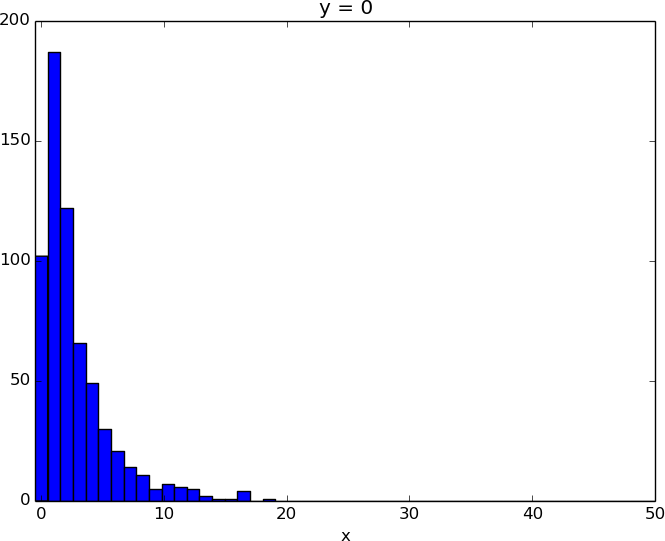
\includegraphics[scale=0.4]{figs/y0.png}
\caption{Values of $A(x, y)$ for $y=0$.}
\label{y0}
\end{subfigure}%
\par\bigskip
\begin{subfigure}{\textwidth}
\centering
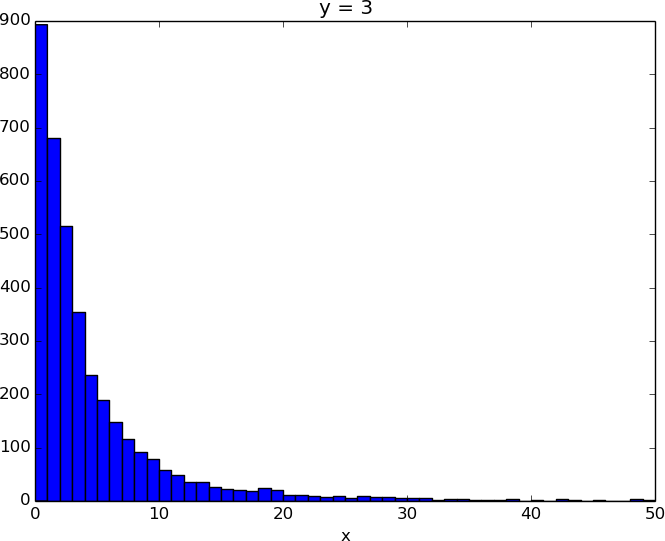
\includegraphics[scale=0.4]{figs/jutarnji1.png}
\caption{Values of $A(x, y)$ for $y=3$.}
\label{jutarnji1}
\end{subfigure}\\[1ex]
\begin{subfigure}{\textwidth}
\centering
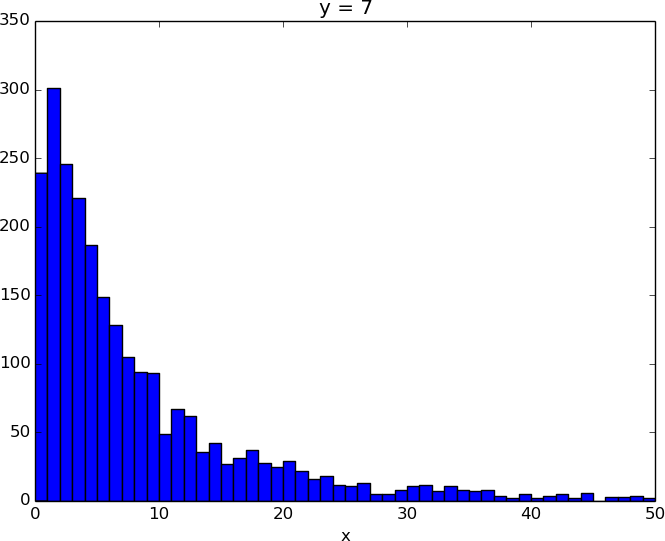
\includegraphics[scale=0.4]{figs/034.png}
\caption{Values of $A(x, y)$ for $y=7$.}
\label{034}
\end{subfigure}
\caption{Values of $A(x,y)$ for fixed $y \in \{0, 3, 7\}$ with respect to number of activations with $x$ neighbours active calculated for the Referendum Dataset.}
\label{fig:test}
\end{figure}

In the  case of information propagation where only social influence is present, graph of activation frequency  with respect to the number of activated neighbours $x$ would look similar to the Figure \ref{y0}. That is, activation frequency for nodes that have at least one activated neighbour will be greater than the number of activations for nodes with $0$ neighbours active.  A certain sign of authority presence is unexpected frequency of activation for nodes that have $0$ activated neighbours. The Figure \ref{jutarnji1} is an example of that kind of activity where frequency of activation with $0$ neighbours active exceed the frequency of activation with $1$ friend active. 

The information propagation dynamic after activation of authority $y=7$ is suspected to be primarily pressured by internal (social influence) what is further approved with Figure \ref{034}. It is important to notice that, as time passes and more nodes become active, the probability of a node having $0$ active neighbours decreases, even for the nodes that become active pressured by external influence. Although the authority $y = 7$ becomes active relatively late, the frequency of activation related to authorities that activate after $y = 7$ form a shape similar to \ref{jutarnji1}. The suspicion of information about the application being propagated mostly pressured by external influence will be confirmed with a model.


\section{Estimating peer and authority coefficients}
Estimation of $\alpha$, $\beta$ and $\gamma$  for the Restricted Referendum dataset gives $\alpha = 0.16432$, $\beta = 0.41826 $ and $\gamma = -8.84820$. The strength of peer and authority influence was obtained by the time-shuffle test based on $1000$ randomized instances of the input graph and the strengths $S_{\alpha} = 0.996$, $S_{\beta} = 0.633$ were obtained. Frequency histograms of estimated $\alpha(D')$ and $\beta(D')$ for randomized datasets $D' \in \mathcal{D}$ used in this test are shown on the Figure \ref{hist_full}. 
\begin{figure}[htp]
\centering
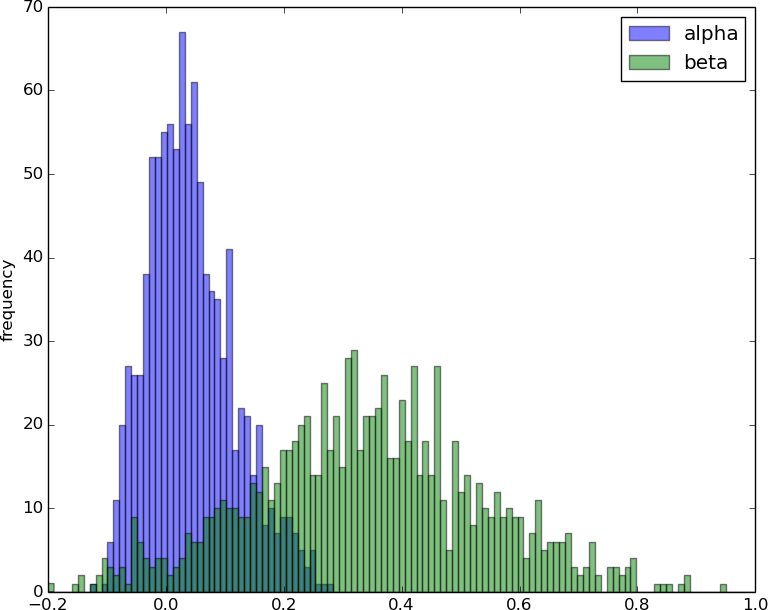
\includegraphics[scale=0.6]{figs/abg1000.png}	
\caption{Frequency histograms of estimated values of $\alpha$ (blue) and $\beta$ (green)  obtained with original version of the model for the Restricted Referendum Dataset with time-shuffle test based on $1000$ randomized instances.}
\label{hist_full}
\end{figure}
								
The estimation algorithm was ran for the Complete Referendum Dataset and the values $\alpha=1.44990$, $\beta=-1.02360$ and $\gamma=-13.52627$ were obtained. The negative value of $\beta$ may lead to conclusion the model, along with its assumptions, is not suitable for  the Complete Referendum Dataset.

The maximum likelihood function for the model was constructed by examining the events of an inactive node 'trying' to activate independently for all time steps and all inactive nodes at that time. To reason about the negative value of $\beta$, the average frequency of activation and average number of trials (observed events) for the duration of time intervals while $y$ authorities were active, along with the corresponding success rate is given in the Table \ref{T1} for the Restricted and in Table \ref{T2} for the Complete Referendum Dataset. Since the frequencies of activation and trials depend on the length of the observed time interval, they were given in the tables as average frequency per time step for every observed time interval. The success rate is observed, since the maximum likelihood estimator tries to fit the distribution model to similarly defined success rate.

\begin{table}[htp]    
\small
%0  0.77791 12549.02 0.062
%1  9.00000 11792.91 0.763
%2  7.34400 11058.83 0.664
%3  3.91023  7636.39 0.512
%4  4.52381  6764.81 0.669
%5  3.74797  6443.38 0.582
\begin{subtable}{\textwidth}
\centering
\begin{tabular}{|c|c|c|c|c|c|c|}
 \hline 
 \rule[-1ex]{0pt}{2.5ex} $y$ & $0$ & $1$ & $2$ & $3$ & $4$ & $5$  \\ 
 \hline 
 \rule[-1ex]{0pt}{2.5ex} successes & $0.77791$ & $9.00000$ & $7.34400$ & $3.91023$ & $4.52381$ & $3.74797$  \\ 
 \hline 
 \rule[-1ex]{0pt}{2.5ex} trials & $12549.02$ & $11792.91$ & $11058.83$ & $7636.39$ & $6764.81$ & $6443.38$ \\ 
 \hline 
 \rule[-1ex]{0pt}{2.5ex} success rate ($10 ^ {-3}$)& $0.062$ & $0.763$ & $0.664$ & $0.512$ & $0.669$ & $0.582$  \\ 
 \hline 
  \hline 
%6  1.26634  5156.96 0.246
%7  0.89345  3001.87 0.298
%8  0.67893  1882.61 0.361
%9  1.41053  1664.66 0.847
%10 3.40826  1434.86 2.375
%11 1.62857   879.45 1.852
 \rule[-1ex]{0pt}{2.5ex} $y$ & $6$ & $7$ & $8$ & $9$ & $10$ & $11$ \\ 
 \hline 
 \rule[-1ex]{0pt}{2.5ex} successes & $ 1.26634$ & $0.89345$ & $0.67893$ & $1.41053$ & $3.40826$ & $1.62857$ \\ 
 \hline 
 \rule[-1ex]{0pt}{2.5ex} trials & $5156.96$ & $3001.87$ & $1882.61$ & $1664.66$ & $1434.86$ & $879.45$ \\ 
 \hline 
 \rule[-1ex]{0pt}{2.5ex} success rate ($10 ^ {-3}$)& $0.246$ & $0.298$ & $0.361$ & $0.847$ & $2.375$ & $1.852$ \\ 
 \hline 
 \end{tabular}  
  \caption{Restricted Referendum Dataset.}
  \label{T1}
 \end{subtable}
\\[1ex]
\begin{subtable}{\textwidth}
\centering
%0 0.77791 1697339.72 0.458
%1 9.00000 1694518.91 5.311
%2 7.34400 1693784.83 4.336
%3 3.91023 1690362.39 2.313
%4 4.52381 1689490.81 2.678
%5 3.74797 1689169.38 2.219
\begin{tabular}{|c|c|c|c|c|c|c|}
 \hline 
 \rule[-1ex]{0pt}{2.5ex} $y$ & $0$ & $1$ & $2$ & $3$ & $4$ & $5$  \\ 
 \hline 
 \rule[-1ex]{0pt}{2.5ex} successes & $0.77791$ & $9.00000$ & $7.34400$ & $3.91023$ & $4.52381$ & $3.74797$  \\ 
 \hline 
 \rule[-1ex]{0pt}{2.5ex} trials & $1697340$ & $1694519$ & $1693785$ & $1690362$ & $1689491$ & $1689169$ \\ 
 \hline 
 \rule[-1ex]{0pt}{2.5ex} success rate ($10 ^ {-6}$)& $0.458$ & $5.311$ & $4.336$ & $2.313$ & $2.678$ & $2.219$  \\ 
 \hline 
  \hline 
 \rule[-1ex]{0pt}{2.5ex} $y$ & $6$ & $7$ & $8$ & $9$ & $10$ & $11$ \\ 
 \hline 
%6  1.26634 1687883 0.750
%7  0.89344 1685728 0.530
%8  0.67893 1684609 0.403
%9  1.41053 1684391 0.837
%10 3.40816 1684161 2.024
%11 1.62857 1639898 0.993
 \rule[-1ex]{0pt}{2.5ex} successes & $ 1.26634$ & $0.89345$ & $0.67893$ & $1.41053$ & $3.40826$ & $1.62857$ \\ 
 \hline 
 \rule[-1ex]{0pt}{2.5ex} trials & $1687883$ & $1685728$ & $1684609$ & $1684391$ & $1684161$ & $1639898$ \\ 
 \hline 
 \rule[-1ex]{0pt}{2.5ex} success rate ($10 ^ {-6}$)& $0.750$ & $0.530$ & $0.403$ & $0.837$ & $2.024$ & $0.993$ \\ 
 \hline 
 \end{tabular}
 \caption{Complete referendum dataset.}
 \label{T2}
\end{subtable}
 \caption{Average frequencies of observed successful activations per time step, average frequencies of trials per time step  and success rates for the time period when $y$ authorities were active on the Restricted and Complete Referendum Datasets.}
\label{tab}
\end{table}

It is important to notice that average frequency of successful events for each time interval stays  the same for both Restricted and Complete Referendum Dataset. Since at each time step only inactive nodes are observed and conducted in trials, it is expected for the averaged frequency of trials to decrease with time as the observed set of nodes shrinks in size. The smaller averaged number of trials for the events observed in late time intervals for the Restricted Referendum Dataset, further induces the growth of success rate as the number of active authorities increases. 

Since there are $99.25\%$ of nodes in the Complete Referendum Dataset that never become active, the number of trials stays roughly the same for the observed time intervals, as seen in the Table \ref{T2}. Therefore the success rate is roughly proportional to the number of successful activations for every interval, \emph{i.e.} it decreases, thus explaining the negative value of $\beta$. 

Since the conducted analysis has shown the proposed model is not suitable for the given Complete Referendum Dataset, the model will be redefined.

\section{Redefining the model of external influence}

The activation of a node without any previously activated neighbours is a pattern attributable  to external influence. To make the proposed model suitable for our purpose, the new definition of attribute  $y$ will be provided.

If $y$ in \eqref{Pxy} were to be defined as the frequency of activated nodes at the observed time step whose neighbours haven't been activated before, the estimated probability distribution will be  expected to increase with $y$. Additionally, thus defined attribute doesn't necessarily have positive correlation with time, unlike the initial definition of $y$. Hence, the errors caused by decreasing number of trials at the end of the observed time for the Restricted Referendum Dataset and the error caused by too many observed nodes that finally don't activate even though maximum number of authorities are active for the Complete Referendum Dataset, have less impact on the results.

Estimation of $\alpha$, $\beta$ and $\gamma$  for the Restricted Referendum Dataset with newly defined model of external influence gives $\alpha = 0.16697$, $\beta = 0.92495$ and $\gamma = -8.60957$. The strength of peer and authority influence was again obtained by the time-shuffle test based on $1000$ randomized instances of the input graph and strengths $S_{\alpha} = 0.018$, $S_{\beta} = 0.959$ were obtained. Frequency histograms of estimated $\alpha(D')$ and $\beta(D')$ of randomized datasets $D' \in \mathcal{D}$ used in this test are shown on the Figure  \ref{hist_full2}. 
\begin{figure}[htp]
\centering
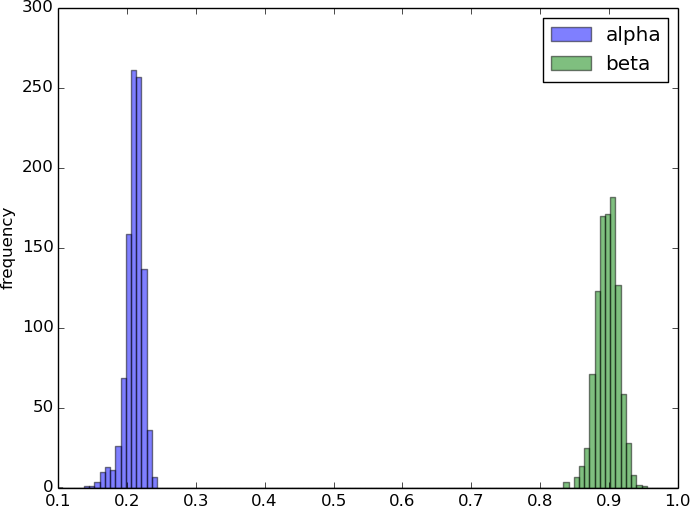
\includegraphics[scale=0.7]{figs/abg1000_2.png}	
\caption{Frequency histograms of estimated values of $\alpha$ (blue) and $\beta$ (green)  obtained with updated version of the model for the Restricted Referendum Dataset with time-shuffle test based on $1000$ randomized instances.}
\label{hist_full2}
\end{figure}
								
The estimation for the Complete Referendum dataset returns $\alpha=0.89215$, $\beta=1.36409$, $\gamma=-15.7230$. The strength of peer and authority influence was again obtained by the time-shuffle test based on $500$ randomized instances of the complete input graph and strengths $S_{\alpha} = 1.000$, $S_{\beta} = 0.998$ were obtained. Frequency histograms of estimated $\alpha(D')$ and $\beta(D')$ of randomized datasets $D' \in \mathcal{D}$ used in this test are shown on the Figure \ref{hist_full3}. 
\begin{figure}[htp]
\centering
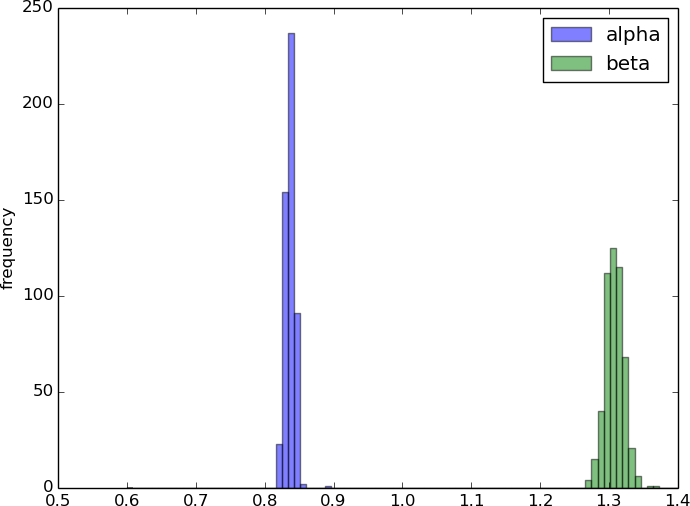
\includegraphics[scale=0.7]{figs/abg500v.png}	
\caption{Frequency histograms of estimated values of $\alpha$ (blue) and $\beta$ (green)  obtained with updated version of the model for the Complete Referendum Dataset with time-shuffle test based on $500$ randomized instances.}
\label{hist_full3}
\end{figure}

\chapter{Conclusion}

The model for information propagation given in \cite{authority} takes into account that information propagation in social networks can be driven by both social (internal) and authority (external) influence. The proposed model is used for determining whether the information item is mainly propagated driven by internal or external influence. The probability of activation for a node that has $x$ active neighbours when $y$ authorities were active is modeled as logistic regression with $3$ parameters, peer influence coefficient $\alpha$, authority influence coefficient $\beta$ and externality coefficient $\gamma$. The logistic regression model is then estimated using the maximal likelihood estimator. Based on the estimated values of $\alpha$ and $\beta$ and  taking into account the results of the randomized test called the time-shuffle test, a decision is made. 

The information propagation analysis for the Referendum Dataset based on the presented model of peer and authority influence has returned estimations for peer and authority coefficients that indicate the model is not suitable for the Referendum Dataset. That is expected since the model assumes the influence of an active node (peer or authority) does not fade away with time which can be easily disproven for the Referendum Dataset.

If the external influence for an inactive node at time $t$ is measured by the number of nodes that activate at that  time and do not have any active neighbours, for estimated peer coefficient $\alpha$ and authority coefficient $\beta$, $0 < \alpha < \beta$ holds on both Restricted and Complete Referendum Dataset. The time shuffle test for the Restricted Referendum Dataset has returned a small value of peer strength and a large value of authority strength. Hence, the information propagation is mainly pressured by external influence. The estimation and the shuffle test for the Complete Referendum Dataset reassures the conclusion is correct. 

\bibliography{literatura}
\bibliographystyle{unsrt}
\pagebreak
\engtitle{Information propagation in online social networks}
\begin{abstract}
In this paper the information propagation model that takes into account both internal (social) and external (authority) influence is presented and revisited. Based on the estimated parameters for the model and the randomization test called time-shuffle test, a decision whether propagation of an information item is mainly peer or authority influence driven can be made. The proposed model and its updated version were used to describe an information item - the existence of the Facebook application referendum2013.hr - as mainly propagated by external (authority) influence. 

\keywords{complex networks,  social networks, information propagation, internal and external influence, peer and authority model,time-shuffle test}
\end{abstract}
\begin{sazetak}
U ovom je radu objašnjen model za širenje informacije  u društvenoj mreži koji uzima u obzir i unutranji (društveni) i vanjski (medijski) utjecaj na širenje informacije. Na temelju predviđenih parametara modela te statističkog testa, moguće je donošenje odluke o načinu širenja promatrane informacije. Točnije, možemo odrediti da li se promatrana informacija više širila pod društvenim ili medijskim utjecajem. Izloženi model te njegova izmijenjena verzija korišteni su za određivanje prirode utjecaja na širenje informacije o postojanju Facebook aplikacije referendum2013.hr. 

\kljucnerijeci{kompleksne mreže, društvene mreže, širenje informacije, model širenja informacije, društveni utjecaj, medijski utjecaj}
\end{sazetak}


\end{document}
